% 原书PDF第38页4.2.2起至第40页4.2.3之前，含原41、42页图。
\subsection{RNA-seq 数据差异表达分析的函数展开方法}

如第4.2.1节所述，RNA-seq 差异表达分析的一种常用策略是：（1）建立读段计数分布的统计模型；（2）基于计数分布模型估计基因的总体表达水平；（3）比较两种条件下总体表达的差异，识别差异表达基因。然而，表达本质上是一个随机过程。内源与外源噪声造成复杂的细胞间基因表达变异。剪接位点、转录起始位点与多聚腺苷酸化位点的使用变化，进一步与生物学变异交织。此外，组织样本含有许多不同类型的细胞，转录起始位置、转录速率与剪接位点都可能因细胞而异。观测读段计数形成依赖于位置的曲线，基因内部的计数模式过于复杂，难以准确、全面地建模。

发展同时考虑读段计数分布、生物学变异与测序技术偏倚的非参数统计方法，有助于改进 RNA-seq 差异表达分析。本节介绍函数展开方法：将碱基层面的读段计数建模为基因组位置的随机表达函数，通过 Karhunen–Loève 分解，将随机函数展开为正交函数主成分（Xiong et al. 2014），并据此构造检验两种条件间差异表达的统计量。

\subsubsection{RNA-seq 数据的函数主成分展开}
先将基因内的读段计数定义为该基因中基因组位置的表达函数。设 $t$ 为某基因组区域内核苷酸的位置，$T$ 为所考察区域的长度。考虑病例与对照两种条件，假设抽取 $n_A$ 名病例与 $n_G$ 名对照，对其 mRNA 测序。病例组第 $i$ 名个体的表达函数 $x_i(t)$，定义为该个体中覆盖基因组位置 $t$ 处核苷酸的读段数。类似地，可定义对照组第 $i$ 名个体的表达函数 $y_i(t)$。

合并病例与对照的表达函数，可以构造正交函数主成分（基函数）$\{\beta_j(t)\}$。由 Karhunen–Loève 展开，$X_i(t)$ 与 $Y_i(t)$ 可写为
\begin{equation}
X_i(t)=\sum_{j=1}^{k}\xi_{ij}\beta_j(t)
\tag{4.109}
\end{equation}
以及
\begin{equation}
Y_i(t)=\sum_{j=1}^{k}\eta_{ij}\beta_j(t),
\tag{4.110}
\end{equation}
其中 $\xi_{ij}=\int_T X_i(t)\beta_j(t)\,dt$，$\eta_{ij}=\int_T Y_i(t)\beta_j(t)\,dt$。$\xi_{ij}$ 与 $\eta_{ij}$ 为互不相关的随机变量，均值为零，方差为 $\lambda_j$，且 $\sum_j\lambda_j<\infty$。以 $\bar\xi_j$ 与 $\bar\eta_j$ 分别表示病例与对照中主成分得分的均值。检验两组间基因差异表达的统计量定义为
\begin{equation}
T_{\mathrm{FPC}}=\frac1{\dfrac1{n_A}+\dfrac1{n_G}}
\sum_{j=1}^{k}\frac{(\bar\xi_j-\bar\eta_j)^2}{S_j},
\tag{4.111}
\end{equation}
其中
\[
S_j=\frac1{n_A+n_G-2}\left[\sum_{i=1}^{n_A}(\xi_{ij}-\bar\xi_j)^2
+\sum_{i=1}^{n_G}(\eta_{ij}-\bar\eta_j)^2\right].
\]
在病例与对照间基因无差异表达的原假设下，$T_{\mathrm{FPC}}$ 渐近服从中心 $\chi^2_{(k)}$ 分布，其中 $k$ 为函数主成分的个数。

\begin{bookexample}{4.6}
为评价泊松分布、负二项分布及 FPCA 拟合 RNA-seq 读段计数的预测准确性，从 GEUVADIS 项目（\url{http://www.ebi.ac.uk/arrayexpress/files/E-GEUV-3/}）提取465个样本中基因 LMNB2 的读段计数，分别用这三种方法拟合。图4.12展示了全部465个样本的观测平均计数曲线及三种方法拟合的平均计数曲线，并展示了观测和拟合的平均总体表达水平。可以看到，虽然 LMNB2 的观测与拟合平均总体表达水平非常接近，三种方法的预测准确性却有很大差别。泊松分布与负二项分布对计数数据的拟合较差，FPCA 的拟合则相当好。
\end{bookexample}
\begin{figure}[p]
\centering
\begin{minipage}{.49\linewidth}\centering
\begin{tikzpicture}[x=1cm,y=1cm]
\node[anchor=south west,inner sep=0] at (0,0) {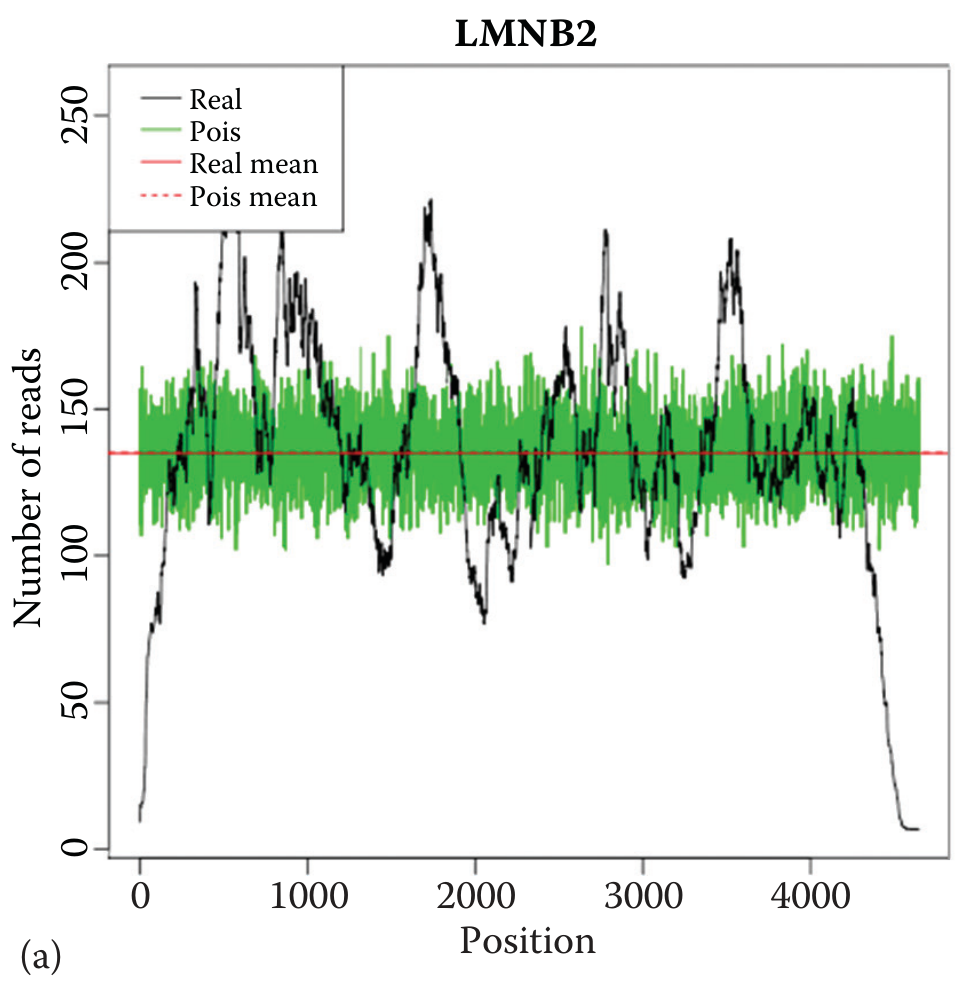
\includegraphics[width=6.7cm]{figures/ch04a_fig12a_data.png}};
\fill[white] (3.1967,0.1284) rectangle (4.2096,0.4590);
\node[inner sep=0pt,fill=white,rotate=0,font=\fontsize{7}{8}\selectfont] at (3.7031,0.2937) {位置};
\fill[white] (0.0011,2.4754) rectangle (0.5168,4.4971);
\node[inner sep=0pt,fill=white,rotate=90,font=\fontsize{7}{8}\selectfont] at (0.1915,3.4862) {读段数};
\fill[white] (1.3000,6.0678) rectangle (1.7268,6.3283);
\node[inner sep=0pt,fill=white,rotate=0,font=\fontsize{6}{8}\selectfont] at (1.5134,6.1980) {观测};
\fill[white] (1.3000,5.8414) rectangle (1.7181,6.1019);
\node[inner sep=0pt,fill=white,rotate=0,font=\fontsize{6}{8}\selectfont] at (1.5091,5.9716) {泊松};
\fill[white] (1.3000,5.6196) rectangle (2.2616,5.8801);
\node[inner sep=0pt,fill=white,rotate=0,font=\fontsize{6}{8}\selectfont] at (1.7808,5.7499) {观测均值};
\fill[white] (1.3000,5.3858) rectangle (2.2529,5.6463);
\node[inner sep=0pt,fill=white,rotate=0,font=\fontsize{6}{8}\selectfont] at (1.7765,5.5161) {泊松均值};
\end{tikzpicture}
\end{minipage}\hfill
\begin{minipage}{.49\linewidth}\centering
\begin{tikzpicture}[x=1cm,y=1cm]
\node[anchor=south west,inner sep=0] at (0,0) {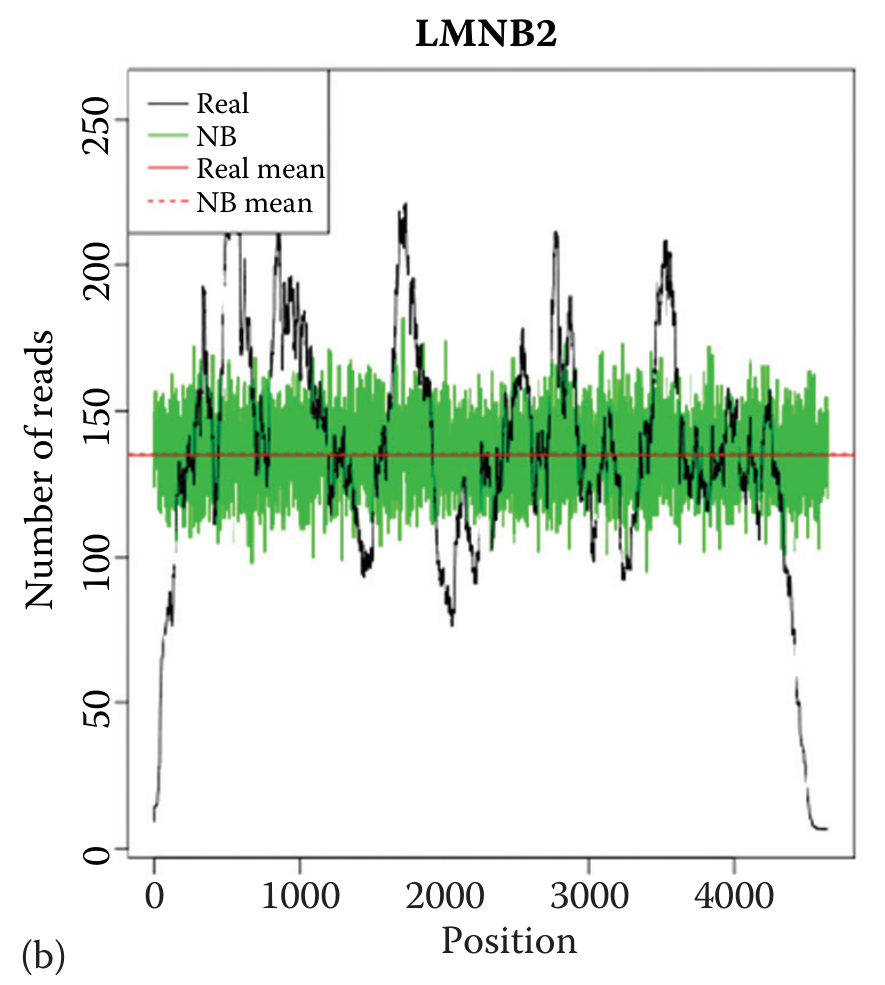
\includegraphics[width=6.7cm]{figures/ch04a_fig12b_data.png}};
\fill[white] (3.3083,0.1405) rectangle (4.3973,0.4933);
\node[inner sep=0pt,fill=white,rotate=0,font=\fontsize{7}{8}\selectfont] at (3.8528,0.3169) {位置};
\fill[white] (0.1099,2.8095) rectangle (0.6478,4.9871);
\node[inner sep=0pt,fill=white,rotate=90,font=\fontsize{7}{8}\selectfont] at (0.3113,3.8983) {读段数};
\fill[white] (1.4573,6.5166) rectangle (1.9139,6.7937);
\node[inner sep=0pt,fill=white,rotate=0,font=\fontsize{6}{8}\selectfont] at (1.6856,6.6551) {观测};
\fill[white] (1.4573,6.2723) rectangle (1.8183,6.5494);
\node[inner sep=0pt,fill=white,rotate=0,font=\fontsize{6}{8}\selectfont] at (1.6378,6.4108) {负二项};
\fill[white] (1.4573,6.0282) rectangle (2.4910,6.3053);
\node[inner sep=0pt,fill=white,rotate=0,font=\fontsize{6}{8}\selectfont] at (1.9742,6.1668) {观测均值};
\fill[white] (1.4573,5.7736) rectangle (2.3954,6.0507);
\node[inner sep=0pt,fill=white,rotate=0,font=\fontsize{6}{8}\selectfont] at (1.9264,5.9121) {负二项均值};
\end{tikzpicture}
\end{minipage}
\par\medskip
\begin{tikzpicture}[x=1cm,y=1cm]
\node[anchor=south west,inner sep=0] at (0,0) {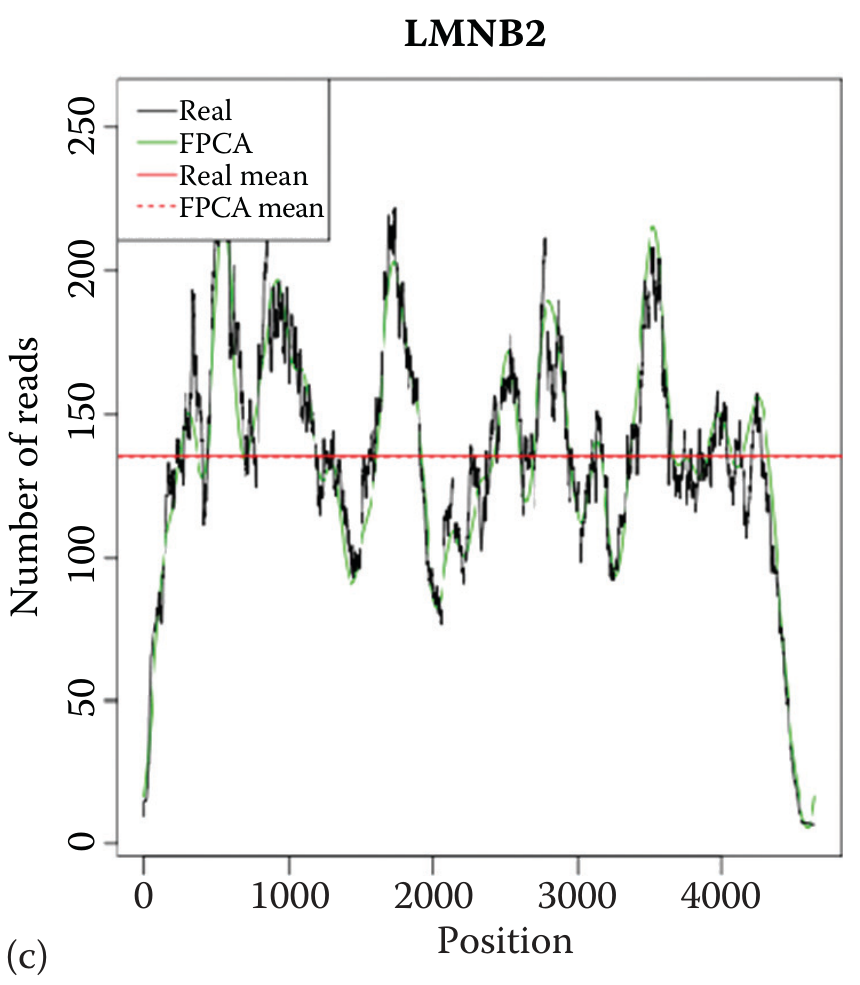
\includegraphics[width=6.7cm]{figures/ch04a_fig12c_data.png}};
\fill[white] (3.3756,0.1453) rectangle (4.4948,0.5069);
\node[inner sep=0pt,fill=white,rotate=0,font=\fontsize{7}{8}\selectfont] at (3.9352,0.3261) {位置};
\fill[white] (0.0003,2.8384) rectangle (0.5469,5.0779);
\node[inner sep=0pt,fill=white,rotate=90,font=\fontsize{7}{8}\selectfont] at (0.2061,3.9581) {读段数};
\fill[white] (1.3665,6.6589) rectangle (1.8348,6.9426);
\node[inner sep=0pt,fill=white,rotate=0,font=\fontsize{6}{8}\selectfont] at (1.6006,6.8007) {观测};
\fill[white] (1.3665,6.3977) rectangle (1.9998,6.6814);
\node[inner sep=0pt,fill=white,rotate=0,font=\fontsize{6}{8}\selectfont] at (1.6831,6.5396) {FPCA};
\fill[white] (1.3665,6.1515) rectangle (2.4287,6.4352);
\node[inner sep=0pt,fill=white,rotate=0,font=\fontsize{6}{8}\selectfont] at (1.8976,6.2933) {观测均值};
\fill[white] (1.3665,5.9024) rectangle (2.5564,6.1861);
\node[inner sep=0pt,fill=white,rotate=0,font=\fontsize{6}{8}\selectfont] at (1.9614,6.0442) {FPCA均值};
\end{tikzpicture}
\origfig{12}{（a）拟合的泊松分布；（b）拟合的负二项分布；（c）用 FPCA 拟合的表达曲线。}
\label{fig:ch04a-12}
\end{figure}


\begin{bookexample}{4.7}
为评价差异表达检验的性能，将 FPCA 与基于总体表达水平的汇总统计量应用于 TCGA 卵巢癌项目的 RNA-seq 数据。该项目对233个卵巢癌组织样本中的15104个基因测序，其中70个样本耐药、163个样本有药物响应。图4.13给出了基因 CHST10 的表达谱。用 FPCA 和总体表达水平（RPKM）检验耐药与药物响应样本间 CHST10 差异表达，所得 $P$ 值分别为0.00003与0.1674；两组总体表达水平的均值差为67.32。图中未见 CHST10 总体表达水平有很大差异，但可以观察到两组表达谱的差异。
\end{bookexample}
\begin{figure}[htbp]
\centering
\begin{tikzpicture}[x=1cm,y=1cm]
\node[anchor=south west,inner sep=0] at (0,0) {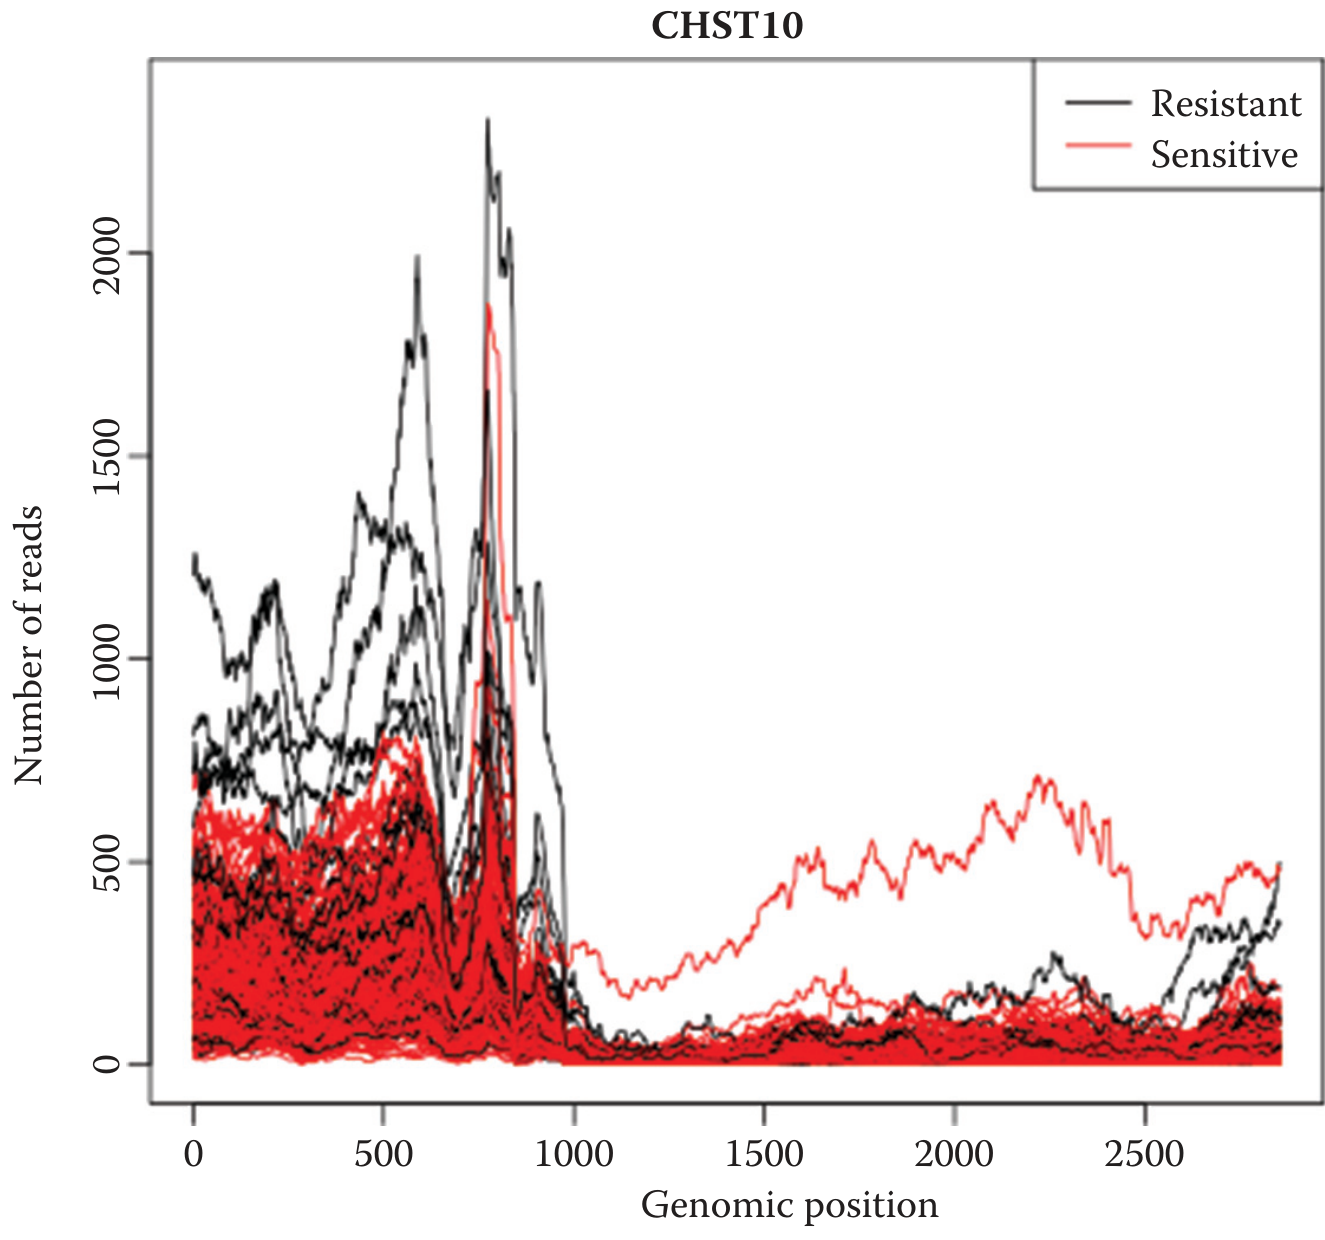
\includegraphics[width=11.3cm]{figures/ch04a_fig13_data.png}};
\fill[white] (5.4362,0.0866) rectangle (8.0365,0.4778);
\node[inner sep=0pt,fill=white,rotate=0,font=\fontsize{8}{8}\selectfont] at (6.7364,0.2822) {基因组位置};
\fill[white] (0.0703,3.8479) rectangle (0.4615,6.2947);
\node[inner sep=0pt,fill=white,rotate=90,font=\fontsize{8}{8}\selectfont] at (0.2659,5.0713) {读段数};
\fill[white] (9.7874,9.4753) rectangle (11.1317,9.8664);
\node[inner sep=0pt,fill=white,rotate=0,font=\fontsize{8}{8}\selectfont] at (10.4595,9.6708) {耐药};
\fill[white] (9.7874,9.0405) rectangle (11.0989,9.4316);
\node[inner sep=0pt,fill=white,rotate=0,font=\fontsize{8}{8}\selectfont] at (10.4432,9.2361) {敏感};
\end{tikzpicture}
\origfig{13}{TCGA 卵巢癌数据集中基因 CHST10 的表达谱。}
\label{fig:ch04a-13}
\end{figure}

\FloatBarrier
